\documentclass[a4paper,11pt]{article}
\input{/home/tof/Documents/Cozy/latex-include/preambule_lua.tex}
\newcommand{\showprof}{show them}  % comment this line if you don't want to see todo environment
\fancyhead[L]{Routage}
\newdate{madate}{10}{09}{2020}
\fancyhead[R]{\displaydate{madate}} %\today
\fancyfoot[L]{~\\Christophe Viroulaud}
\fancyfoot[C]{\textbf{Page \thepage}}
\fancyfoot[R]{\includegraphics[width=2cm,align=t]{/home/tof/Documents/Cozy/latex-include/cc.png}}

\begin{document}
\begin{Form}
\begin{commentprof}
\textbf{MATÉRIEL: ficelles, 4 papiers destination (Périgueux, Bordeaux, Pékin, Athènes), 15 papiers messages, 15 papiers "accusé de réception", 15 enveloppes, rouleau PQ}
\end{commentprof}
\section{Problématique}
Chaque ordinateur est repéré par son adresse IP sur le réseau. En prenant exemple sur le service de \emph{La Poste} il semble donc aisé de transmettre un message à un destinataire pour peu que l'on connaisse son adresse.
\begin{center}
\shadowbox{\parbox{15cm}{\centering Quel système dans le réseau internet tient le rôle du facteur et de ses intermédiaires?}}
\end{center}
\section{Des matériels et des protocoles}
\subsection{Un dispositif central}
Les réseaux internes ont une topologie en étoile. Chaque réseau est relié aux autres par une topologie maillée. Les nœuds qui composent ce maillage sont \emph{les routeurs}.
\begin{figure}[!h]
\centering
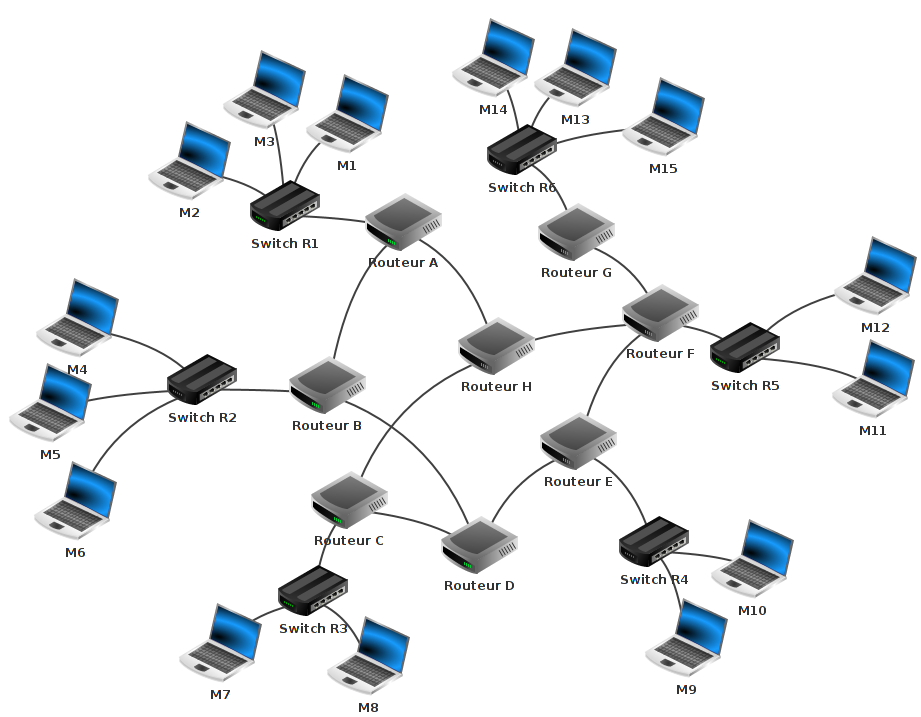
\includegraphics[width=7cm]{ressources/routage.png}
\captionof{figure}{Le réseau internet}
\label{routage}
\end{figure}
\begin{activite}
\begin{enumerate}
\item Sur la figure \ref{routage} entourer un réseau interne.
\item Dans un réseau interne, quel dispositif relie les ordinateurs entre eux?
\item Quels sont les avantages d'utiliser une topologie maillée pour internet?
\end{enumerate}
\end{activite}
\begin{commentprof}
un switch est relié à un routeur (les 2 sont inclus dans votre box) pour accéder à internet.
\end{commentprof}
\subsection{Transmettre au bon destinataire}
\begin{activite}
Réaliser la simulation puis établir les étapes du protocole IP. 
\end{activite}
\begin{commentprof}
Techniquement dans le réseau interne, ce sont d'autres protocoles qui interviennent (avec adresse MAC notamment).\\ on ne regarde que le réseau internet.\\message dans enveloppe et marquer nom de la destination (au crayon)\\mettre un routeur en panne si le message passe toujours par lui.
\end{commentprof}
\subsection{Garantir l'intégrité des données}
\begin{activite}
Réaliser la nouvelle simulation puis établir les étapes du protocole TCP. 
\end{activite}
\begin{commentprof}
accusé de réception\\mais lui aussi peut se perdre --> chrono\\préparer les accusés numérotés\\plusieurs paquets avec même numéro pour renvoi\\dans la réalité, on peut expliquer le principe de l'accusé de réception "le plus haut"\\
Algorithme pour la source :
\begin{enumerate}
\item Quand la source envoie un paquet, elle lance son minuteur.
\item Si la source reçoit l’accusé de réception avant l’expiration du minuteur, c’est terminé, le paquet peut être effacé par la source.
\item Si le minuteur expire avant réception de l’accusé de réception, la source recommence à l’étape "renvoi du paquet et relance du minuteur".
\end{enumerate}
    
\end{commentprof}
\begin{commentprof}
\section*{Retour historique}
\end{commentprof}
\begin{commentprof}
\section{À chaque situation son protocole}
Le protocole \emph{UDP (User Datagram Protocol)} peut également être encapsulé dans IP. Il est plus simple à mettre en pratique car il ne propose pas de système d'accusé de réception.
\end{commentprof}
\end{Form}
\end{document}